\documentclass[oneside, draft]{epstfg}

\usepackage{lipsum}
\usepackage[numbers]{natbib}
\usepackage{fancysprefs}
\usepackage{booktabs}
\usepackage{wrapfig}
\usepackage{enumitem}
\usepackage{xfrac}
\usepackage{multirow}

\usepackage{tikz}

\usetikzlibrary{arrows}
\usetikzlibrary{patterns}
\usetikzlibrary{intersections}
\usetikzlibrary{calc}
\usetikzlibrary{fadings}

\definecolor{palette1}{HTML}{1B9E77}
\definecolor{palette2}{HTML}{D95F02}
\definecolor{palette3}{HTML}{7570B3}
\definecolor{palette4}{HTML}{E7298A}
\definecolor{palette5}{HTML}{66A61E}
\definecolor{palette6}{HTML}{E6AB02}
\definecolor{palette7}{HTML}{A6761D}
\definecolor{palette8}{HTML}{666666}

\tikzstyle{vnlin}=[rectangle, inner sep=0pt, minimum height=6pt, minimum width=0pt, draw, fill=black]
\tikzstyle{hnlin}=[rectangle, inner sep=0pt, minimum height=0pt, minimum width=6pt, draw, fill=black]
\tikzset{>=latex}

\bibliographystyle{abbrv}

\title[spa]{Monitorización, captura y almacenamiento inteligente de tráfico de red a 40Gbps}
\title[eng]{Monitoring, capture and smart storage of network traffic at 40 Gbps}
\author{Guillermo Julián Moreno}
\tutor{Francisco Gómez Arribas}
\date[spa]{Mayo 2016}
\date[eng]{May 2016}
\group[spa]{HPCN}
\group[eng]{HPCN}
\department[spa]{Departamento}
\department[eng]{Department}

\setdegreeDouble

\begin{abstract}[spa]
\lipsum[1]
\end{abstract}

\begin{abstract}[eng]
\lipsum[2]
\end{abstract}

\keywords[spa]{keyword, comma, separated, list}
\keywords[eng]{keyword, comma, separated, engl}

\newacronym[longplural = {Centros de Proceso de Datos}]{cpd}{CPD}{Centro de Proceso de Datos}
\newacronym{gbps}{Gbps}{Gigabits por segundo}
\newacronym{nic}{NIC}{Tarjeta de Interfaz de Red}
\newacronym{irq}{IRQ}{Petición de interrupción}
\newacronym{api}{API}{\textit{Application Programming Interface}}
\newacronym{SPAN}{SPAN}{\textit{Switched Port ANalyzer}}
\newacronym{BPF}{BPF}{\textit{Berkeley Packet Filter}}

\newglossaryentry{10gbe}{
	name = {10 GbE},
	description = {Estándares de transmisión de datos sobre Ethernet a 10 gigabits por segundo}}

\newglossaryentry{NAPI}{
	name = {NAPI},
	description = {``New API'', una API de Linux desarrollada para mitigar interrupciones en \textit{drivers} de red y mejorar el rendimiento bajo condiciones de alta carga}}

\newglossaryentry{driver}{
	name = {Driver},
	text ={\textit{driver}},
	description = {También llamado controlador de dispositivo, es un programa que permite al sistema operativo interactuar con un periférico hardware}}

\newglossaryentry{jumbo}{
	name = {Paquete jumbo},
	text={paquete jumbo},
	description = {Paquetes Ethernet de tamaño superior a 1500 bytes}}

\newglossaryentry{DMA}{
	name = {DMA},
	description = {Direct Memory Access, un sistema que permite a los periféricos acceder directamente a la memoria del sistema}
}

\newglossaryentry{padding}{
	name = {Padding},
	text = {\textit{padding}},
	description = {Datos ``de relleno'' que se añaden a una estructura de datos para alinearla a un tamaño concreto}
}

\newglossaryentry{RAID}{
	name = {RAID},
	description = {\textit{Redundant Array of Independent Disks}, una tecnología de virtualización de almacenamiento de datos que combina múltiples discos en una única unidad virtual, mejorando rendimiento y/o redundancia}
}

\newglossaryentry{RSS}{
	name = {RSS},
	description = {\textit{Receive Side Scaling}, una tecnología para \textit{drivers} de red que permite distribuir de forma eficiente los paquetes recibidos entre varias CPUs}
}

\newglossaryentry{RoCE}{
	name = {RoCE},
	description = {\textit{RDMA over Converged Ethernet}, tecnología de Mellanox para permitir acceso directo a memoria remota (RDMA) a través de redes Ethernet}
}

\begin{document}

\selectlanguage{spanish}

\frontmatter

\maketitle[spa]
\maketitle[eng]

\makeinnertitle[spa]
\makeinnertitle[eng]

\makeabstract[spa]
\makeabstract[eng]

\tableofcontents
\clearsidepage
\listoftables
\clearsidepage
\listoffigures
\clearsidepage

\mainmatter

\chapter{Introducción y motivación}

Durante los últimos años, las necesidades de ancho de banda de Internet se han ido multiplicando a una velocidad difícil de imaginar en su momento. Muchos \glspl{cpd} ya han desplegado redes \gls{10gbe}, y los dispositivos capaces de funcionar a 40 \gls{gbps} o incluso a 100 \gls{gbps} ya están disponibles comercialmente.

Por supuesto, junto con las nuevas redes de alta velocidad llega la necesidad de monitorizarlas, ya sea para diagnosticar problemas, detectar intrusiones o asegurar un nivel de calidad de servicio. Sin embargo, los sistemas operativos modernos no están totalmente preparados para el manejo de estas velocidades. Incluso para \gls{10gbe} se hacen necesarias configuraciones específicas \cite{leitao2009tuning} que permitan al sistema alcanzar las tasas que ofrece el hardware.

Para sortear las limitaciones de los sistemas operativos en este sentido son necesarias soluciones específicas y dedicadas. En muchos casos se emplean sistemas o tarjetas de red diseñadas a tal efecto, aunque el coste es mayor que soluciones software basadas en sistemas y tarjetas estándar.

Dentro de las soluciones de monitorización por software hay dos aspectos que muchas  no contemplan: el de marcado de paquetes o \textit{timestamping} y el del orden de captura. A 40 Gbps, el tiempo entre paquetes puede llegar a ser de 13 nanosegundos\footnote{Tomando paquetes de tamaño mínimo, 64 bytes, y añadiendo el \textit{interframe gap} de 8 bits.}. Una recepción desordenada o imprecisiones mínimas en las marcas de tiempo pueden ser decisivas para que una herramienta de análisis detecte o ignore anomalías en el tráfico; o para que dé falsos positivos a raíz de fallos en la captura. Teniendo en cuenta que estos problemas ya los introducen las propias redes y sistemas a monitorizar, es necesario reducirlos todo lo posible en el lado de la captura.

\section{Objetivos}

Este trabajo se plantea resolver el problema de la monitorización de tráfico en redes 40 GbE, ampliando el sistema de captura HPCAP \cite{victorPhD}, desarrollado en el grupo de investigación HPCN (Escuela Politécnica Superior, UAM) por Víctor Moreno. Para ello, los objetivos a cumplir serán los siguientes:

\begin{itemize}[itemsep=0pt]
\item Estudiar los límites de la arquitectura ya existente de HPCAP e identificar los puntos de mejora.
\item Plantear una solución que permita la captura de tráfico a tasa de línea junto con marcas de tiempo precisas.
\item Desarrollar métodos que hagan posible el almacenamiento de información sobre el tráfico que pueda ser analizada posteriormente.
\item Crear un entorno de pruebas que permita verificar y probar el rendimiento de sistemas de captura de tráfico de alta velocidad.
\end{itemize}

\chapter{Estado del arte}

A lo largo de esta sección se estudiarán las soluciones actuales de captura de tráfico a alta velocidad, empezando antes con una introducción al funcionamiento de \textit{drivers} de red que permita identificar los cuellos de botella que los sistemas de monitorización deberán evitar.

\section{Funcionamiento y cuellos de botella de un \textit{driver} de red}
\label{sec:EstadoArte:Funcionamiento}

\begin{figure}[hbtp]
\centering
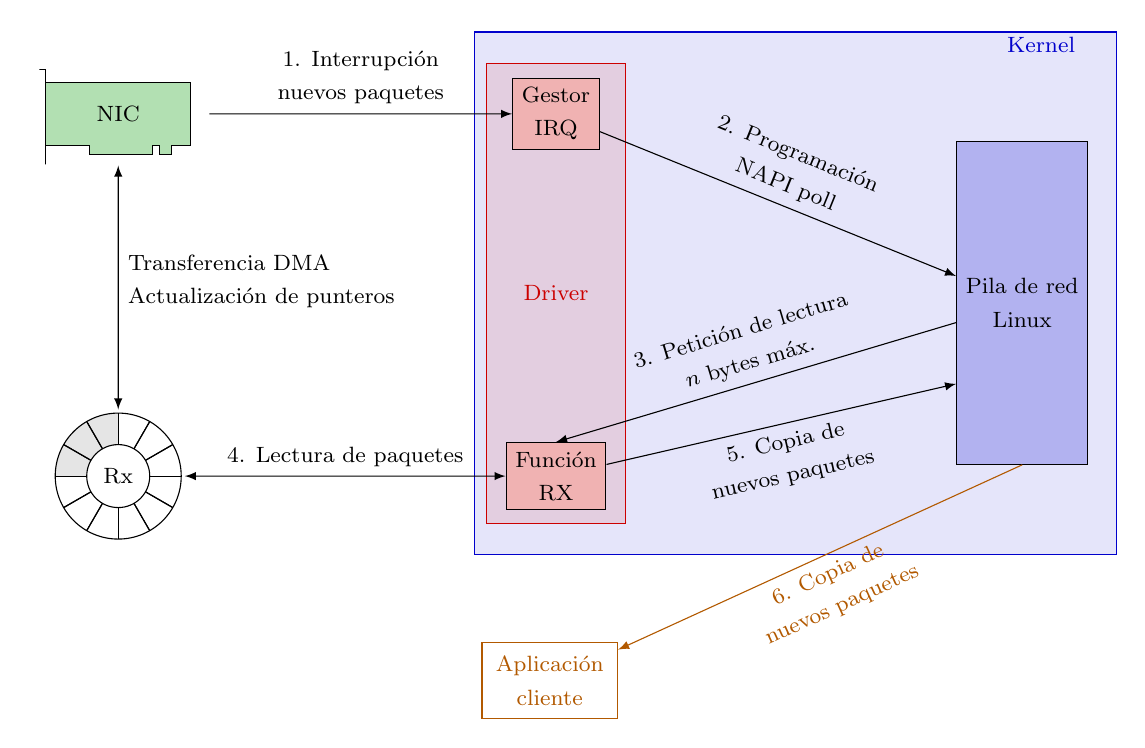
\begin{tikzpicture}[font = {\fontsize{8pt}{12}\selectfont}, scale = 0.8]
\begin{scope}[yshift = 4cm]
\draw[fill = green!60!black, fill opacity = 0.3] (-0.1, 1.2) -- (0, 1.2) -- (0,-0.3) -- (0,0) -- (0.7,0) -- (0.7,-0.15) -- (1.7, -0.15) -- (1.7, 0) -- (1.8, 0) -- (1.8, -0.15) -- (2, -0.15) -- (2,0) -- (2.3, 0) -- (2.3, 1) -- (0,1) -- (0, 1.2) -- cycle ;

\node[rectangle, minimum width = 2.3cm, minimum height = 1cm] (NIC) at (1.15, 0.5) {NIC};
\end{scope}

\draw[blue!80!black, fill = blue!80!black, fill opacity = 0.1] (6.8, 5.8) rectangle (17, -2.5);
\node[blue!80!black] at (15.8, 5.6) {Kernel};

\draw[red!80!black, fill = red!80!black, fill opacity = 0.1] (7, 5.3) rectangle (9.2, -2);
\node[red!80!black] at (8.1, 1.65) {Driver};

\node[draw, fill = red!80!black!30!white, align = center] (IRQ) at (8.1, 4.5) {Gestor \\ IRQ};
\node[draw, fill = blue!80!black!30!white, minimum height = 4.1cm, minimum width = 1.5cm, align = center] (KRN) at (15.5, 1.5) {Pila de red \\ Linux};
\node[draw, align = center, fill = red!80!black!30!white] (POLL) at (8.1, -1.25) {Funci\'on \\ RX};

\node[draw, orange!70!black, align = center, inner sep = 5pt] (APP) at (8, -4.5) {Aplicaci\'on \\ cliente};

\coordinate (KRN-Mid) at ($(KRN.west)!0.5!(KRN.south west)$);

\begin{scope}[xshift = 1.15cm, yshift = -1.25cm, rotate = 90]
\fill[gray!20!white] (0,0) -- (0,1) arc (90:0:1cm) -- cycle;
\foreach \x in {0, 30, ..., 360}
	\draw ({cos(\x)}, {sin(\x)}) -- ({-cos(\x)}, {-sin(\x)});
\draw (0,0) circle [radius = 1cm];
\draw[black, fill = white] (0,0) circle [radius = 0.5cm]; % Poor man's \clip for intersecting regions
\node[circle, inner sep = 0.45cm] (RNG) at (0,0) {Rx};
\end{scope}

\draw[->] (NIC) --
	node[midway, above, align = center, sloped] {1. Interrupci\'on \\ nuevos paquetes}
	(IRQ);

\draw[->] (IRQ) --
	node[midway, above, sloped, align = center] {2. Programaci\'on \\ NAPI poll}
	(KRN);

\draw[->] (KRN) --
	node[midway, above, sloped, align = center] {3. Petici\'on de lectura \\ $n$ bytes m\'ax.}
	(POLL.north);

\draw[<->, shorten <= 0.15cm] (NIC) --
	node[midway, right, align = left] {Transferencia DMA \\ Actualizaci\'on de punteros}
	(RNG);

\draw[<->] (POLL) -- node[midway, above, align = center, sloped] {4. Lectura de paquetes}
	(RNG);

\draw[->] (POLL) --
	node[midway, below, align = center, sloped] {5. Copia de \\ nuevos paquetes}
	(KRN-Mid);

\draw[<-, orange!70!black] (APP) --
	node[midway, below, sloped, align = center] {6. Copia de  \\ nuevos paquetes}
	(KRN.south);
\end{tikzpicture}

\caption[Funcionamiento de un \textit{driver} de red en Linux]{Esquema del funcionamiento de un \gls{driver} de red en Linux. En rojo, las funciones pertenecientes al \gls{driver}.}
\label{fig:LinuxNetworkStack}
\end{figure}

A grandes rasgos, el funcionamiento de un \textit{\gls{driver}} de red en Linux es el que aparece en la \fref{fig:LinuxNetworkStack}. Cuando la \gls{nic} recibe nuevos paquetes, emite una \gls{irq} que es recibida por la función correspondiente configurada por el \gls{driver}. Éste se comunica con la pila de red del \textit{kernel} de Linux, más concretamente con el subsistema \gls{NAPI} \cite{NAPI}, avisando de la disponibilidad de nuevos paquetes. Además, desactivará las interrupciones de la tarjeta hasta que no se hayan leído todos los paquetes pendientes, para mejorar así el rendimiento.

El subsistema \gls{NAPI} programará una llamada a la función de recepción del \gls{driver} en función de la carga del sistema, pidiendo la lectura de hasta un cierto máximo de bytes. Cuando esa llamada se realice, el \gls{driver} leerá de una región de memoria los paquetes que la tarjeta haya copiado a través de transferencias DMA, y los transferirá a la pila de red de Linux, que a su vez los gestionará y distribuirá a las aplicaciones cliente correspondientes.

Si bien esta arquitectura es muy efectiva para un sistema de propósito general, tiene varias desventajas como sistema de captura de alto rendimiento. Por un lado, se introduce una cierta latencia al tener que esperar a la primera interrupción y a la llamada correspondiente del subsistema NAPI para empezar a leer los paquetes del anillo de recepción de la tarjeta. Por otra, se realizan dos copias redundantes: del anillo de recepción a la pila de red de Linux y de ésta a la aplicación cliente.

\section{Sistemas de captura de tráfico}

Para el sistema operativo Linux se pueden encontrar multitud de sistemas de captura de tráfico. Entre los más conocidos se puede encontrar \textit{libpcap} y sistemas basados en él, como \textit{tcpdump} o \textit{Wireshark}. Ahora bien, estos sistemas no están preparados para la captura a altas tasas de tráfico, por lo que surgen nuevos sistemas más eficientes y con mejor rendimiento. A lo largo de esta sección revisaremos algunos de ellos.

\subsection{Linux PACKET\_MMAP}

Una opción para captura de alto rendimiento integrada en el propio \textit{kernel} de Linux es la configuración llamada PACKET\_MMAP. Esta opción permite acceder directamente a los anillos de recepción del sistema desde espacio de usuario, de tal forma que no hay que realizar llamadas a sistema ni hacer copias adicionales para recibir cada paquete.

Aunque es un método más eficiente que la captura paquete a paquete, se sigue usando la pila de red de Linux, lo que hace difícil la mejora y modificación para obtener mayor rendimento o poder usar los marcados de tiempo \textit{hardware} que ofrezca la tarjeta.

\subsection{PF\_RING ZC}

PF\_RING ZC (\textit{Zero Copy}) es la versión modificada de PF\_RING DNA \cite{rizzo201210}. Se trata de un sistema comercial de captura de tráfico a 10 Gbps preparado para procesar y reenviar paquetes copiando sólo los datos de la \gls{nic} a la memoria de sistema, saltándose la pila de red del sistema. Una de sus principales fortalezas es la virtualización: PF\_RING ZC permite a máquinas virtuales sobre Linux acceder al tráfico a 10 Gbps, e incluso realiazr operaciones sin copias de memoria entre esas máquinas virtuales para mejorar el rendmiento.

Sin embargo, todavía no ofrece captura a 40 Gbps, marcado de tiempo preciso o soporte para NICs distintas de las de Intel.

\subsection{DPDK}

Desarrollado por --- entre otros --- Intel, DPDK (\textit{Data Plane Development Kit}) \cite{IntelDPDK} es un conjunto de librerías y \textit{drivers} para el envío y procesado de paquetes a alta velocidad. Soporta tarjetas de múltiples fabricantes, incluyendo Mellanox e Intel; y permite captura a 40 Gbps con \glspl{nic} apropiadas.

DPDK expone una \gls{api} que permite a las aplicaciones configurar el sistema de captura y recibir tráfico. También se pueden usar herramientas ya desarrolladas, como MoonGen \cite{emmerich2015moongen} que permite generar y recibir paquetes usando programas Lua interpretados en tiempo real.

La principal desventaja de DPDK es que obliga al programador a realizar cualquier tarea adicional a la captura en espacio de usuario, de tal forma que resulta difícil aplicar marcas de tiempo precisas al no poder detectar el momento exacto en el que llega cada paquete.

\subsection{HPCAP}

HPCAP \cite{victorPhD} es un sistema de captura desarrollado en el grupo HPCN de la Escuela Politécnica Superior (UAM) por Víctor Moreno, que permite la captura de tráfico a alta velocidad con marcado de tiempo preciso; y que además está optimizado para permitir el almacenamiento de ese tráfico en disco para su posterior análisis.

El sistema consiste en la modificación del \gls{driver} original de Intel para tarjetas \gls{10gbe}, de tal forma que los paquetes capturados no pasan por la pila de red del sistema sino que se guardan en un \textit{buffer} intermedio en memoria del sistema. Las aplicaciones cliente podrán leerlos y procesarlos a través de la \gls{api} que expone HPCAP, o realizar un guardado directo a disco sin copias adicionales.

\chapter{Desarrollo e implementación}

\section{Arquitectura de los \textit{drivers} originales}
\label{sec:ArquitecturaOriginal}

\begin{figure}[btp]
\centering
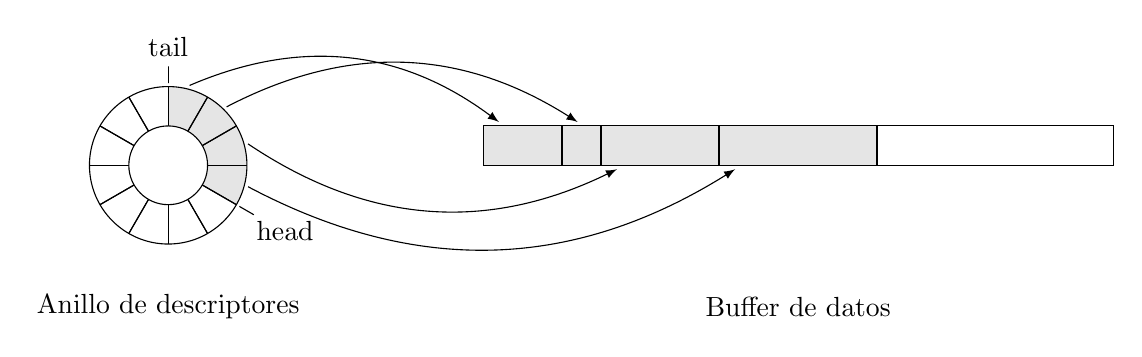
\begin{tikzpicture}
\fill[gray!20!white] (0,0) -- (0,1) arc (90:-30:1cm) -- cycle;
\foreach \x in {0, 30, ..., 360}
	\draw ({cos(\x)}, {sin(\x)}) -- ({-cos(\x)}, {-sin(\x)});
\draw (0,0) circle [radius = 1cm];
\draw[black, fill = white] (0,0) circle [radius = 0.5cm]; % Poor man's \clip for intersecting regions

\node[vnlin, label = {above:tail}] at (0,1.15) {};

\node[hnlin, label = {below right:head}, rotate = -30] at ({1.15 * cos(-30)}, {1.15 * sin(-30)}) {};

\node at (0, -1.8) {Anillo de descriptores};
\node at (8, -1.8) {Buffer de datos};

\fill[gray!20!white] (4, 0) rectangle (9, 0.5);
\draw (4, 0) rectangle (12,0.5);

\draw[thick] (5, 0) -- (5, 0.5);
\draw[thick] (5.5, 0) -- (5.5, 0.5);
\draw[thick] (7, 0) -- (7, 0.5);
\draw[thick] (9, 0) -- (9, 0.5);

\draw[->] ({1.05 * cos(75)}, {1.05 * sin(75)}) to [bend left] (4.2, 0.55);
\draw[->] ({1.05 * cos(45)}, {1.05 * sin(45)}) to [bend left] (5.2, 0.55);
\draw[->] ({1.05 * cos(15)}, {1.05 * sin(15)}) to [bend right] (5.7, -0.05);
\draw[->] ({1.05 * cos(-15)}, {1.05 * sin(-15)}) to [bend right] (7.2, -0.05);

\end{tikzpicture}

\caption[Esquema del anillo de descriptores para recepción de paquetes]{Esquema del anillo de descriptores para la recepción de paquetes. Cada descriptor tiene un puntero a los datos del paquete recibido y un campo que marca si el descriptor tiene o no datos. En gris, los datos y descriptores listos para ser leídos por el \gls{driver}.}
\label{fig:DriverRings}
\end{figure}

Para poder adaptar HPCAP a las \glspl{nic} de 40 Gbps de Intel y Mellanox es necesario utilizar los \glspl{driver} originales de los fabricantes y modificarlos para que sea el código de HPCAP el encargado de la recepción. Esto implica conocer su funcionamiento no sólo a grandes rasgos (\fref{sec:EstadoArte:Funcionamiento}), sino también las rutinas de comunicación con el hardware y de reserva de recursos de esos \glspl{driver} originales.

A pesar de ser de fabricantes distintos, los dos \glspl{driver} siguen el mismo proceso para inicializarse y para la recepción de paquetes. Cuando el \gls{driver} se inserta en el sistema Linux, lee los parámetros de configuración de la línea de comandos y empieza a reservar recursos acorde a esos parámetros. Entre esos recursos están las regiones de memoria de los anillos de recepción, donde la \gls{nic} escribirá los paquetes recibidos; y estructuras en memoria compartida entre software y hardware, de donde se leerán datos como los descriptores de paquetes y los punteros de cabecera y cola del anillo.

El anillo de descriptores es la estructura de datos que permite la transferencia de paquetes desde la \gls{nic} al \gls{driver}. Cada descriptor de paquete es una estructura de tamaño fijo que contiene una variable con el estado del descriptor, con los marcadores que determinan si tiene datos, si ha tenido algún error o si es parte de un \gls{jumbo}; y un puntero a los datos del paquete de red correspondiente, que han sido copiados a la memoria del sistema por la \gls{nic}.

Este anillo se comporta como una cola, aunque el acceso se realiza de manera distinta. El puntero de cabecera, \textit{head}, que marca hasta dónde hay paquetes pendientes de leer, no se actualiza por la \gls{nic} al enviar nuevos paquetes al sistema. En su lugar, para comprobar si hay o no nuevos paquetes por leer, el \gls{driver} simplemente lee el campo de estado del siguiente descriptor de paquete para saber si tiene datos o no.

La rutina de recepción, llamada por el subsistema \gls{NAPI}, va leyendo ese anillo de descriptores y enviando los nuevos paquetes que encuentra al sistema operativo, que se encargará de repatirlos a su destino correspondiente.

Una vez que los paquetes se han leído, no sólo hay que actualizar el puntero de cola, sino también notificar al sistema \gls{DMA} de que la memoria que usaban queda libre para su uso por la tarjeta. Realizar esta operación paquete por paquete introduce un coste adicional que se puede ahorrar acumulando varias operaciones que se realizan de una vez, aunque no deben acumularse demasiadas para evitar que la \gls{nic} se quede sin descriptores donde copiar nuevos paquetes y los descarte.

Por lo tanto, para que HPCAP funcione con estos \glspl{driver}, la principal modificación a hacer es sustituir la rutina de recepción original. Para ello, se evita el registro de la interfaz en el subsistema \gls{NAPI}, se desactivan las interrupciones de la \gls{nic}, y se lanzan los hilos de recepción de HPCAP cuando el resto del \gls{driver} se haya inicializado correctamente.

\section{Recepción a 40 Gbps}
\label{sec:Desarrollo:Recepcion40Gbps}

Tal y como se comentaba en la introducción, la recepción a 40 Gbps es un desafío importante por las restricciones de tiempo. A esta tasa, los paquetes pueden llegar cada 13 nanosegundos, lo que en un procesador de gama alta a 3,40 GHz apenas significan 44 ciclos.

\begin{wraptable}[8]{l}[1.5cm]{0.35\textwidth}
\vspace{-15pt}
\begin{tabular}{lc}
\toprule
\textbf{Operación} & \textbf{Ciclos} \\ \midrule
Acceso caché L1 & 4 \\
Acceso caché L2 & 12 \\
Acceso caché L3 & 44 \\
\textit{Branch mispredict} & 16 \\ \bottomrule
\end{tabular}
\caption{Latencias en CPUs Intel con arquitectura Skylake \cite{intelOptimization}.}
\label{tab:LatenciaIntelSkylake}
\end{wraptable}

Esta restricción de tiempo hace imposible que un único hilo pueda soportar toda la carga de tráfico. Un fallo de caché o del predictor de saltos puede consumir un cuarto del tiempo disponible para el procesado de un paquete, de tal forma que es prácticamente imposible procesar los paquetes a esa tasa incluso aunque no hubiese que copiarlos después a un \textit{buffer} intermedio.

Así, se hace necesario el uso de varios hilos de lectura que sí puedan soportar conjuntamente estas altas tasas de tráfico. El problema a resolver será el de la concurrencia y sincronización entre hilos en tres puntos clave:

\begin{enumerate}[itemsep=0pt, topsep = 0pt]
\item Lectura de paquetes del anillo de recepción.
\item Devolución ordenada de los descriptores leídos a la tarjeta.
\item Copia al \textit{buffer} intermedio de HPCAP.
\end{enumerate}

Por supuesto, todas las operaciones de sincronización tendrán que hacerse sin mecanismos de bloqueo, que son demasiado lentos para el procesado a tasa de 40 Gbps. A priori, la solución sería la implementación de una cola sin bloqueos (por ejemplo, \cite{krizhanovsky2013lock}). Sin embargo, esta situación específica y las características de los lectores y de los clientes que accederán al \textit{buffer} intermedio de HPCAP permitirán la simplificación de las operaciones y la reducción de los mecanismos de concurrencia necesarios.

\subsection{Lectura del anillo de recepción}

A la hora de la lectura, un problema a tener en cuenta es el de la caché. Un fallo de caché puede provocar una latencia de muchos ciclos de reloj (\fref{tab:LatenciaIntelSkylake}), y con ello la pérdida de paquetes. Si todos los hilos de recepción tratan de leer todos los paquetes del anillo de recepción, los patrones de acceso no van a ser predecibles. Cuando un hilo acceda a un descriptor, el sistema cargaría en la caché de su núcleo descriptores cercanos para un acceso más rápido. Ahora bien, es posible que el resto de hilos consuman esos paquetes, de tal forma que el siguiente paquete disponible ya no estaría cargado en caché y habría una latencia adicional al acceder a él.

\begin{wrapfigure}[9]{R}{0.3\textwidth}
\centering
\vspace{-20pt}
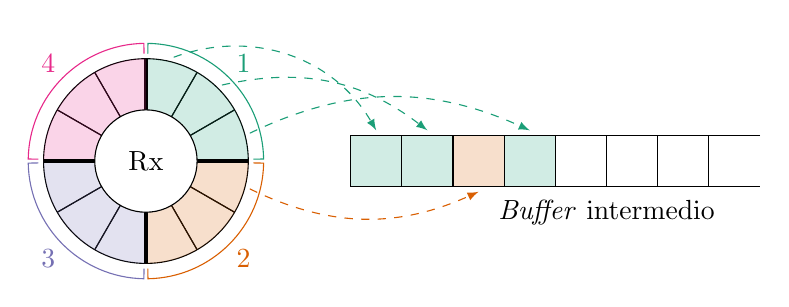
\begin{tikzpicture}[scale = 1.3]
\foreach \x in {0, 30, ..., 360}
	\draw ({cos(\x)}, {sin(\x)}) -- ({-cos(\x)}, {-sin(\x)});
\draw (0,0) circle [radius = 1cm];


\foreach[count = \i] \x/\c in {90/palette1, 0/palette2, -90/palette3, -180/palette4} {
	\draw[\c]
		({1.05 * cos (\x - 1)}, {1.05 * sin (\x - 1)})
		-- ({1.15 * cos (\x - 1)}, {1.15 * sin (\x - 1)})
		arc ({\x - 1}:{\x - 90 + 1}:1.15cm)
		-- ({1.05 * cos (\x - 90 + 1)}, {1.05 * sin (\x - 90 + 1)});

	\fill[opacity = 0.2, \c] (0,0) -- ({cos(\x)}, {sin(\x)})
		arc ({\x}:{\x - 90}:1cm) -- (0,0);

	\node[\c] at ({1.35 * cos (\x - 45)}, {1.35 * sin (\x - 45)}) {\i};

	\draw[very thick] (0,0) -- ({cos(\x)}, {sin(\x)});
}

\draw[black, fill = white] (0,0) circle [radius = 0.5cm]; % Poor man's \clip for intersecting regions
\node at (0,0) {Rx};

\fill[palette1, opacity = 0.2] (2, -0.25) rectangle (3, 0.25);
\fill[palette2, opacity = 0.2] (3, -0.25) rectangle (3.5, 0.25);
\fill[palette1, opacity = 0.2] (3.5, -0.25) rectangle (4, 0.25);

\foreach[count = \i] \x in {0,1,...,6} {
	\draw ({2 + \x / 2}, -0.25) rectangle ({2.5 + \x / 2}, 0.25);
}

\node at (4.5, -0.5) {\textit{Buffer} intermedio};

\draw (6, 0.25) -- (5.5, 0.25) -- (5.5, -0.25) -- (6, -0.25);
\node at (5.8, 0) {$\dotsb$};

\draw[palette1, dashed, ->] ({1.05 * cos (75)}, {1.05 * sin (75)}) to[bend left = 40] (2.25, 0.3);
\draw[palette1, dashed, ->] ({1.05 * cos (45)}, {1.05 * sin (45)}) to[bend left = 25] (2.75, 0.3);
\draw[palette2, dashed, ->] ({1.05 * cos (-15)}, {1.05 * sin (-15)}) to[bend right = 25] (3.25, -0.3);
\draw[palette1, dashed, ->] ({1.05 * cos (15)}, {1.05 * sin (15)}) to[bend left = 25] (3.75, 0.3);


\end{tikzpicture}

\caption{División del anillo de recepción en cuatro segmentos fijos para los hilos.}
\label{fig:RingAssignment}
\end{wrapfigure}

Para evitar este problema, a cada hilo de lectura se le asigna un segmento fijo del anillo de recepción como en la \fref{fig:RingAssignment}. De esta forma cada hilo siempre accederá a los mismos descriptores, lo que permitirá incluir instrucciones de \textit{prefetch} para garantizar en la medida de lo posible que los datos a acceder estén siempre en la caché.

Esta asignación fija de segmentos del anillo también evita problemas de concurrencia, ya que no hay competición por acceso a los mismos recursos.

Por último, se minimiza el desorden en la lectura. Si todos los hilos leyesen los mismos descriptores, lo más probable es que los paquetes se copien en un orden distinto al que tenían cuando llegaron a la tarjeta. Sin embargo, de esta forma los hilos copian secuencialmente la mayor parte de los paquetes, y sólo se produciría desorden cuando haya dos o más hilos con paquetes pendientes al mismo tiempo. Con tasas bajas de paquetes por segundo, esto apenas ocurrirá durante pequeños intervalos de tiempo.

\subsection{Devolución ordenada de los descriptores leídos}

El siguiente problema a resolver es el de la devolución ordenada de los descriptores ya leídos y de las regiones de memoria correspondiente a la tarjeta, para que ésta los pueda reutilizar para los nuevos paquetes que lleguen. Es importante que esta devolución se realice por lotes al ser más eficiente. Además, ha de ser secuencial: no se pueden dejar atrás descriptores sin devolver ya que pueden provocar fallos de segmentación o la tarjeta los puede sobreescribir antes de tiempo.

Al segmentar el anillo de recepción, esta tarea se simplifica considerablemente y no son necesarios mecanismos de sincronización complejos. Cada hilo puede liberar los descriptores de su segmento por lotes sin problemas: la única restricción es que ya se hayan liberado todos los descriptores del segmento anterior.

La solución implementada es la siguiente. A cada hilo se le asignan dos variables, \texttt{can\_free} y \texttt{freed\_last\_rxd}. La primera variable indica si el hilo puede liberar sus descriptores, y la segunda si ya ha liberado el último de los descriptores de su segmento. A la hora de liberar los descriptores, se hace la primera comprobación sobre \texttt{can\_free}: si es 1, se liberan sin problemas. Además, si se llega al último descriptor, \texttt{freed\_last\_rxd} se pone a 1 y \texttt{can\_free} a 0 (hay que esperar, de nuevo, a que el segmento anterior libere sus descriptores).

Si, por otra parte, \texttt{can\_free} es 0, se lee la variable \texttt{freed\_last\_rxd} del segmento previo. Si es 1, indica que ya se pueden liberar los descriptores del segmento actual, así que se resetea su valor a 0 y \texttt{can\_free} se pone a 1. Es necesario que esta comprobación se haga sólo cuando \texttt{can\_free} sea 0. El pseudocódigo de este procedimiento se puede ver en el \fref{lst:AlgoritmoDescriptores}.

\begin{algorithm}[hbtp]
\begin{algorithmic}
\Function{free\_descriptors}{thread, descr}
\State prev $\gets$ \Call{previous\_thread\_of}{thread}
	\If{can\_free[thread] == 0 \&\& freed\_last\_rxd[prev] == 1}
		\State freed\_last\_rxd[prev] $\gets$ 0
		\State can\_free[thread] $\gets$ 1
		\State \Call{read\_barrier}{\ }
	\EndIf

	\If{can\_free[thread] == 1}
		\State \Call{release\_to\_nic}{descr}

		\If{\Call{is\_last\_in\_segment}{descr, thread}}
			\State \Call{write\_barrier}{\ }
			\State freed\_last\_rxd[prev] $\gets$ 1
			\State can\_free[thread] $\gets$ 0
		\EndIf
	\EndIf
\EndFunction
\end{algorithmic}
\caption{Algoritmo de liberación de descriptores}
\label{lst:AlgoritmoDescriptores}
\end{algorithm}

La única técnica de concurrencia usada es que la variable \texttt{freed\_last\_rxd} ha de ser atómica, de tal forma que su valor está constantemente sincronizado entre todos los hilos y no hay posibilidad de que un hilo la lea mientras otro está escribiendo su valor. Además, para mantener un orden estricto en la lectura y escritura de las estructuras de datos.

\subsection{Copia al \textit{buffer} intermedio de HPCAP}

El último problema a resolver es el de la copia al \textit{buffer} intermedio de HPCAP, de donde leerán después los clientes. Para ello se empleará una variable atómica que marque la siguiente posición de escritura en el \textit{buffer}. Cuando un hilo quiera escribir un nuevo paquete, aumentará esa variable en el tamaño del paquete más la cabecera correspondiente, reservando ese espacio a la vista del resto de hilos. Una vez hecha esa reserva, escribirá los datos y continuará con el siguiente paquete.

En un principio, habría que asegurar que esta variable se mantuviese entre 0 y el tamaño del \textit{buffer} de escritura, pero esto implicaría no una operación atómica (sumar un valor y leer el resultado) sino varias, ya que habría que calcular el módulo si el valor obtenido supera el tamaño del \textit{buffer}. Esto implicaría más mecanismos de sincronización y por lo tanto un rendimiento menor.

Por suerte, se puede aprovechar el desbordamiento de enteros de C para hacer ese módulo implícitamente. Por el diseño de HPCAP, el tamaño del \textit{buffer} intermedio es siempre una potencia de 2, luego se puede dejar que la variable atómica desborde normalmente y después calcular el módulo tamaño del \textit{buffer} para obtener la posición real, ya que $(x \mod 2^{32}) \mod 2^n = x \mod 2^n$, donde $2^n$ es el tamaño del \textit{buffer} con $n ≤ 32$.

El siguiente paso es notificar a los clientes que hay nuevos datos disponibles para leer. De nuevo, se pueden aprovechar cuestiones de diseño de HPCAP para evitar mecanismos extra de concurrencia. En una cola sin bloqueos habría que evitar de alguna forma que los clientes puedan leer datos que no se han terminado de escribir. Sin embargo, en HPCAP los clientes están en espacio de usuario, y eso induce un retardo que hace innecesarios más mecanismos de sincronización.

El peor caso ocurriría cuando un hilo actualiza la variable reservando espacio para un nuevo paquete, y justo en el ciclo siguiente se lee esa variable en otro hilo desde una llamada \texttt{ioctl}. Ahora bien, para que ese valor leído llegue a espacio de usuario primero ha de realizarse una copia a la memoria de espacio de usuario y se tiene que hacer un cambio del modo \textit{kernel} a modo espacio de usuario para que la aplicación cliente retome el control de la ejecución, lo que habitualmente lleva más de 50 nanosegundos, unos 170 ciclos de reloj a 3,40 GHz. En ese tiempo se asegura que la copia se ha realizado correctamente, dado que los hilos de lectura no son interrumpidos en ningún momento. Así, incluso en el caso en el que menos tiempo pasaría desde la reserva del espacio de escritura hasta que la aplicación cliente lea esos datos queda garantizado que la copia se realiza correctamente.

\paragraph{Detección de llenado del \textit{buffer}} Es necesario asegurarse de que, al copiar los paquetes, no se sobreescriben datos que todavía no hayan leído los clientes. Dado que las reservas de tamaño se hacen de forma atómica, no es posible comprobar si hay espacio y luego hacer la reserva: podría darse una condición de carrera en la que, habiendo espacio para un único paquete, dos hilos comprueben a la vez que tienen espacio suficiente y por lo tanto sobreescriban el \textit{buffer}.

La solución es una limitación \textit{a priori} de la cantidad de datos que puede copiar cada hilo. Antes de entrar en el bucle de lectura, cada hilo comprueba el espacio libre $e$ en el \textit{buffer} (distancia entre desplazamientos de escritura y lectura) y calcula el límite de datos a copiar como $\sfrac{e}{n}$, donde $n$ es el número de hilos. De esta forma, la condición de carrera anterior desaparece: si no hay espacio para un paquete, al dividir ese espacio entre $n$ hilos ninguno de ellos lo copiará al \textit{buffer} y por lo tanto no habrá sobreescritura.

Además, esta solución no afecta al rendimiento: mientras el \textit{buffer} no esté cerca de llenarse, el coste de salir del bucle de lectura y recalcular el espacio libre es mínimo en comparación con el tiempo invertido en leer y copiar todos los paquetes. Si por otra parte el \textit{buffer} está cerca de llenarse, cada hilo acabaría llenando aproximadamente la misma $n$-ésima parte del espacio restante antes de comprobar que no hay más espacio y salir del bucle.

\paragraph{\textit{Padding}} Hay que tener en cuenta que el propósito de HPCAP es la captura y guardado en disco de los paquetes, y este es el principal caso de uso a optimizar.

Precisamente para facilitar esas copias de \textit{buffer} a ficheros, HPCAP implementa un \gls{padding} \cite{MorenoTFM2012} de tal forma que la aplicación cliente siempre pueda copiar un número entero de paquetes en archivos con un tamaño exacto de 2 GB, sin dejar paquetes cortados entre fichero y fichero. Esto permite maximizar el rendimiento del \gls{RAID} y del acceso a memoria (las lecturas y escrituras siempre están alineadas a tamaño de bloque) y usar ciertas opciones que mejoran el rendimiento.

En esta versión, por lo tanto, hay que seguir manteniendo el \gls{padding} para que las copias a disco sigan siendo óptimas, aunque el método para insertarlo tiene que cambiar. La implementación original mantenía un desplazamiento dentro del fichero, que se actualizaba cada vez que se copiaba un paquete. En el momento de la copia, comprobaba primero si el paquete a copiar entraba dentro del tamaño de fichero. Si no lo hacía, se incluía una cabecera marcando la longitud del \gls{padding} reiniciando el desplazamiento dentro del fichero a cero, y a continuación copiando el paquete.

\begin{figure}[tbp]
\centering
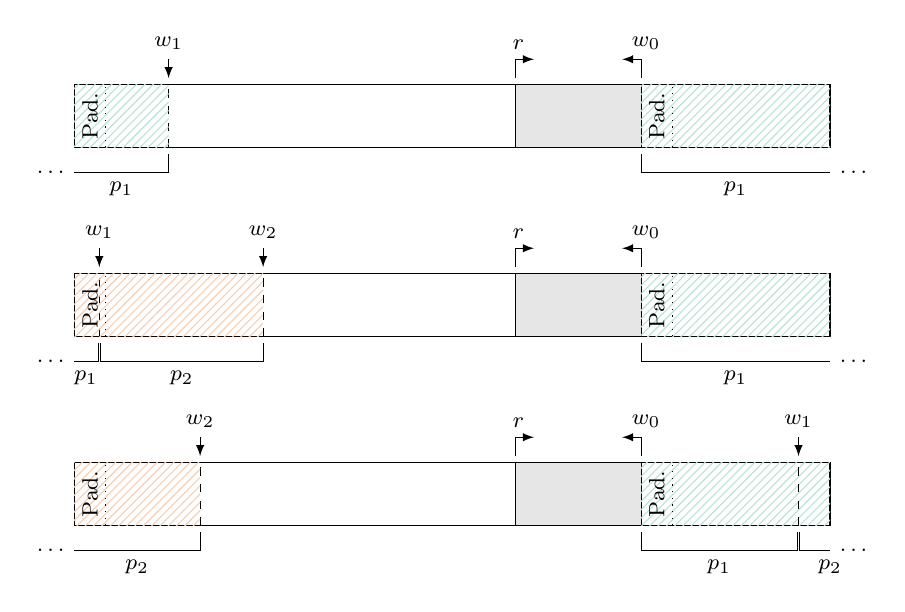
\begin{tikzpicture}[scale = 0.8, font = \footnotesize]

\begin{scope}[yshift = -3cm]
\draw (0,0) rectangle (12, 1);

\draw[->] (7, 1.1) |- (7.3, 1.4) node[above left] {$r$};
\draw[->] (9, 1.1) |- (8.7, 1.4) node[above right] {$w_0$};

\draw[fill = gray, fill opacity = 0.2] (7,0) rectangle (9,1);

\fill[pattern = north east lines, pattern color = palette1!30!white] (9,0) rectangle (12, 1);

\node[rotate = 90] at (9.25, 0.5) {Pad.};
\draw[dotted] (9.5, 0) -- (9.5, 1);

\draw (9, -0.1) -- (9, -0.4) -- node[midway, below] {$p_1$} (11.48, -0.4) -- (11.48, -0.1);

\draw[<-] (11.5, 1.1) -- (11.5, 1.4) node[above] {$w_1$};
\draw[dashed] (11.5, 0) -- (11.5, 1);

\draw (11.52, -0.1) -- (11.52, -0.4) -- (12, -0.4) node[right] {$\dots$} node[below] {$p_2$}  ;
\draw (0, -0.4) node[left] {$\dots$} -- (2, -0.4) node[midway, below] {$p_2$} -- (2, -0.1);

\draw[<-] (2, 1.1) -- (2, 1.4) node[above] {$w_2$};
\draw[dashed] (2, 0) -- (2, 1);

\fill[pattern = north east lines, pattern color = palette2!30!white] (0,0) rectangle (2, 1);
\node[rotate = 90] at (0.25, 0.5) {Pad.};
\draw[dotted] (0.5, 0) -- (0.5, 1);
\end{scope}

\begin{scope}[yshift = 0cm]
\draw (0,0) rectangle (12, 1);

\draw[->] (7, 1.1) |- (7.3, 1.4) node[above left] {$r$};
\draw[->] (9, 1.1) |- (8.7, 1.4) node[above right] {$w_0$};

\draw[fill = gray, fill opacity = 0.2] (7,0) rectangle (9,1);

\fill[pattern = north east lines, pattern color = palette1!30!white] (9,0) rectangle (12, 1);

\node[rotate = 90] at (9.25, 0.5) {Pad.};
\draw[dotted] (9.5, 0) -- (9.5, 1);

\draw (9, -0.1) -- (9, -0.4) -- node[midway, below] {$p_1$} (12, -0.4) node[right] {$\dots$};

\draw (0, -0.4) node[left] {$\dots$} -- (0.38, -0.4) node[midway, below] {$p_1$} -- (0.38, -0.1);

\draw[<-] (0.4, 1.1) -- (0.4, 1.4) node[above] {$w_1$};
\draw[dashed] (0.4, 0) -- (0.4, 1);

\fill[pattern = north east lines, pattern color = palette2!30!white] (0,0) rectangle (3, 1);
\node[rotate = 90] at (0.25, 0.5) {Pad.};
\draw[dotted] (0.5, 0) -- (0.5, 1);

\draw[<-] (3, 1.1) -- (3, 1.4) node[above] {$w_2$};
\draw[dashed] (3, 0) -- (3, 1);
\draw (0.42, -0.1) -- (0.42, -0.4) -- node[midway, below] {$p_2$} (3, -0.4) -- (3, -0.1);
\end{scope}


\begin{scope}[yshift = 3cm]
\draw (0,0) rectangle (12, 1);

\draw[->] (7, 1.1) |- (7.3, 1.4) node[above left] {$r$};
\draw[->] (9, 1.1) |- (8.7, 1.4) node[above right] {$w_0$};

\draw[fill = gray, fill opacity = 0.2] (7,0) rectangle (9,1);

\fill[pattern = north east lines, pattern color = palette1!30!white] (9,0) rectangle (12, 1);

\node[rotate = 90] at (9.25, 0.5) {Pad.};
\draw[dotted] (9.5, 0) -- (9.5, 1);

\draw (9, -0.1) -- (9, -0.4) -- node[midway, below] {$p_1$} (12, -0.4) node[right] {$\dots$};

\draw (0, -0.4) node[left] {$\dots$} -- (1.5, -0.4) node[midway, below] {$p_1$} -- (1.5, -0.1);

\draw[<-] (1.5, 1.1) -- (1.5, 1.4) node[above] {$w_1$};
\draw[dashed] (1.5, 0) -- (1.5, 1);

\fill[pattern = north east lines, pattern color = palette1!30!white] (0,0) rectangle (1.5, 1);
\node[rotate = 90] at (0.25, 0.5) {Pad.};
\draw[dotted] (0.5, 0) -- (0.5, 1);
\end{scope}

\end{tikzpicture}

\caption[Esquema de implementación del \textit{padding} en el \textit{buffer} intermedio]{Esquema de implementación de \textit{padding}. En el primer caso, el mismo hilo escribe el \gls{padding} a principio y final de fichero. En el segundo y tercer no tiene espacio para escribirlo al principio, por lo que se completa al escribir otro paquete.}
\label{fig:BufferPadding}
\end{figure}

Tal y como se ha diseñado la escritura concurrente, es imposible implementar el \gls{padding} de la misma forma, ya que siempre se reserva el tamaño del paquete tanto si cabe en el fichero actual como si no. La solución al problema será llenar ese espacio ya reservado con \gls{padding}, teniendo en cuenta que es posible que no haya espacio para la cabecera completa al principio o al final del fichero. Una vez terminada esa escritura, se reservará de nuevo espacio para copiar el paquete que se iba a copiar en un principio y se continuará normalmente con el proceso.

Dado que el desplazamiento dentro del \textit{buffer} se guarda sin hacer el módulo, no hace falta mantener otro contador separado para el desplazamiento dentro del fichero. Para obtenerlo, sólo es necesario calcular ese desplazamiento módulo el tamaño del fichero. La única precaución a tener es que el tamaño del fichero ha de ser divisor del máximo valor de la variable ($2^{32}$ bytes, 4 GB).

Ese desplazamiento permitirá al \gls{driver} detectar cuándo, una vez reservado el espacio en el \textit{buffer}, el paquete a copiar no entra por completo en el fichero y es necesario insertar un \gls{padding}. El primer paso es comprobar si en el espacio restante del fichero entra el paquete que está pendiente de escribir y además otra cabecera adicional. Es necesario tener en cuenta la inclusión de esa cabecera adicional para evitar casos en los que no quede espacio siquiera en el fichero para una cabecera completa que marque el \gls{padding}.

Si no hay espacio suficiente, se introduce una cabecera con los marcadores de tiempo a 0 y que indique la longitud del \gls{padding}, en este caso, hasta el final de fichero. Además, se comprueba si desde el principio del fichero hasta la última posición reservada ($w_1$ en la \fref{fig:BufferPadding}) hay espacio suficiente para incluir otra cabecera de \gls{padding}. Si lo hay, ese mismo hilo escribirá la cabecera y después se continuará la escritura de paquetes con normalidad.

Si por el contrario no se puede incluir la cabecera a comienzo de fichero, la siguiente escritura (que puede ser realizada por ese mismo hilo o por otro cualquiera, es indiferente) se encargará de hacerlo. Para ello, se comprueba si la diferencia entre el inicio del fichero y la primera posición en la que hay que escribir ($w_1$) es menor que la longitud de cabecera, en cuyo caso se introduce ese \gls{padding} a comienzo de fichero, que llegará hasta la última posición que se había reservado ($w_2$ en la \fref{fig:BufferPadding}).

\subsection{Marcas de tiempo}

Dado que la tarjeta sobre la que se ha diseñado y probado el \textit{driver} ofrece marcado de todos los paquetes en el propio hardware, se puede evitar el marcado de tiempo software, que sería más impreciso al depender del rendimiento de cada hilo y su velocidad para leer descriptores de la tarjeta. Así también se evita marcar los paquetes de forma desordenada, ya que un hilo puede empezar a leer y marcar paquetes antes de que el hilo anterior haya podido acabar con todos los de su segmento.

Para obtener las marcas de tiempo, durante la configuración inicial de la tarjeta se activa el filtrado hardware. En la recepción, cada descriptor incluirá un marcado de tiempo usando un reloj interno de la tarjeta, que después habrá que convertir a la hora local y guardar en la cabecera del paquete en un formato legible con toda la precisión posible, que en el caso de la tarjeta de Mellanox implica almacenarlo en nanosegundos.

\subsection{Ajustes del hardware y configuración}
\label{sec:Desarrollo:AjustesHardware}

Además de la arquitectura de hilos para alto rendimiento, es necesario cambiar la configuración de la tarjeta para optimizar la tasa de recepción. Por defecto, las tarjetas están preparadas para recepción con múltiples anillos (tecnología \gls{RSS}), distribuyendo los paquetes o incluso realizando operaciones como la eliminación de cabeceras VLAN.

Ahora bien, todas estas características no son necesarias si el objetivo es capturar todo el tráfico usando la menor cantidad de recursos posible. Esas operaciones adicionales bajan el rendimiento y es necesario desactivarlas. En particular, se realizan las siguientes modificaciones:

\begin{itemize}[itemsep = 0pt]
\item Se desactiva \gls{RSS} para paquetes UDP.
\item Se reduce el número de colas \gls{RSS} a 1, y se configura la función más rápida (\textit{XOR}) para la distribución.
\item Se desactivan los modos \gls{RoCE} y de descarga de VLAN.
\item Se activa el modo de \gls{RSS} estático, que da mejor rendimiento a costa de menor flexibilidad en las reglas de distribución.
\end{itemize}

\section{Almacenamiento del tráfico: filtrado y guardado selectivo}

En la sección anterior se ha expuesto un diseño para la recepción de tráfico a 40 Gbps, pero falta considerar las opciones disponibles para poder almacenar todo ese tráfico para su posterior análisis.

La opción directa, el almacenamiento de todo el tráfico, no es factible si se quieren mantener unos costes bajos. Como se puede ver en la \fref{tab:Desarrollo:CosteAlmacenamiento}, incluso para un entorno de captura conservador (24 horas de tráfico almacenado a 20 Gbps) los costes son excesivamente altos. La única opción factible serían discos mecánicos, y aún faltaría tener en cuenta el coste del sistema RAID que soporte como mínimo 36 discos.

\begin{table}[b!tp]
\centering
\begin{tabular}{cl cccc}
\toprule
\textbf{Tipo} & \textbf{Modelo} & \textbf{Velocidad} & \textbf{Capacidad} & \textbf{Nº Discos} & \textbf{Coste} \\
& & \textbf{(MB/s)} & \textbf{(TB)} & & \textbf{\texteuro} \\
\midrule
\multirow{2}{*}{SSD}
	& Samsung 850 Pro 	& 520 & 2 	& 106 &  86,496 \texteuro \\[0.2em]
	& Intel DC 3700 	& 970 & 1.6 & 132 & 158,400 \texteuro \\[0.4em]
\multirow{2}{*}{Mecánico}
	& HGST Ultrastar  	& 220 & 6 	&  36 &  21,600 \texteuro \\[0.2em]
	& Seagate Entrp.	& 240 & 4   &  53 &  26,500 \texteuro \\[0.2em]
\bottomrule
\end{tabular}
\caption{Estimaciones de coste de los discos necesarios para un sistema de captura de 24 horas de tráfico a 20 Gbps.}
\label{tab:Desarrollo:CosteAlmacenamiento}
\end{table}

Se hace necesario por lo tanto desarrollar sistemas que permitan filtrar el tráfico recibido o guardar sólo la información estrictamente necesaria de cada paquete. A lo largo de esta sección se planteará el diseño de estas soluciones para el filtrado.

\subsection{Filtrado de paquetes}

Dado que el filtrado ha de hacerse en el bucle de recepción, es necesario que el sistema sea simple y se puedan evaluar los filtros rápidamente. Para ello, se traslada toda la complejidad al espacio de usuario, donde se traducirán los filtros deseados a una estructura de datos que simplifique el análisis.

Esta estructura será una lista de cadenas y su correspondiente posición de inicio en el paquete. Un elemento de esa lista podría ser, por ejemplo, la cadena que contenga la dirección MAC \texttt{AA:BB:CC:DD:EE:FF} y la posición de inicio 0, de tal forma que el filtro aceptaría sólo paquetes con esa MAC destino.

Además, se podrá configurar el filtrado para que sólo se acepte un paquete si todas las cadenas coinciden, o configurar cadenas con coincidencia inversa (esto es, que se rechace un paquete si la cadena coincide). De esta forma se pueden implementar numerosos filtros comunes, como filtrado por destino/origen (incluyendo puertos TCP/UDP) o incluso protocolo de la capa de aplicación.

La principal ventaja de este diseño es su simplicidad y su buen rendimiento, como se verá en la sección de validación experimental. Ahora bien, es un sistema poco flexible y los filtros pueden no ser correctos cuando las cabeceras de los paquetes varíen de tamaño: por ejemplo, no se podría hacer un filtro capaz de aceptar paquetes TCP con y sin cabecera VLAN (la cabecera VLAN añade bytes extra antes de la cabecera TCP).

Una posible solución a esa falta de flexibilidad sería permitir la creación de filtros anidados, de tal forma que se pueda implementar cualquier combinación lógica deseada. Sin embargo, eso implicaría una complejidad mayor en el bucle de recepción y por lo tanto un peor rendimiento. Además, sería más difícil traducir los filtros deseados a la combinación de cadenas y configuración necesarias para llevarlos a cabo.

La otra solución sería integrar el \textit{driver} con los filtros \gls{BPF} integrados en el \textit{kernel} Linux. Estos filtros se programan usando una sintaxis específica (por ejemplo, \texttt{host 192.168.1.1}) que se traduce a un lenguaje máquina específico. El código resultante se ejecuta en un intérprete optimizado dentro del \textit{kernel}. Si bien es un sistema complejo para filtros sencillos, es apropiado para casos más genéricos al tener un lenguaje máquina fácilmente interpretable y además el compilador ya está preparado para los distintos protocolos y cabeceras de tamaño variable que puedan encontrarse.

\paragraph{Configuración de filtros ``en vivo''}

Para evitar paradas innecesarias en la captura, el diseño del sistema de filtros permite la configuración ``en vivo'', esto es, sin dejar en ningún momento de capturar paquetes. Tal y como se comentaba en secciones anteriores, las necesidades de rendimiento del bucle de recepción impiden técnicas de sincronización especialmente complejas.

La activación de los filtros se controlará así con una variable atómica. Para activar los filtros, primero se rellenarán las estructuras correspondientes a través de una llamada \texttt{ioctl}, y después se pondrá a 1 la variable de control, de tal forma que los hilos sólo entren en el filtro cuando ya está listo para ser ejecutado.

Si el filtro ya se encuentra activado, primero se desactiva la variable de control y se esperan 1000 nanosegundos, para dar tiempo suficiente a todos los hilos a salir de la rutina de comprobación de filtros. Una vez pasado ese tiempo, se modifican los filtros y se reactivará la variable de control tal y como se ha descrito anteriormente.

\subsection{Almacenamiento selectivo}

En combinación con el filtrado, se pueden seleccionar ciertos datos del paquete a guardar para reducir la tasa efectiva a procesar posteriormente. Un primer enfoque sería implementar una limitación del tamaño de paquete capturado, tal y como se hace en otras herramientas de captura. Así, sólo se guardarían como mucho los $n$ primeros bytes de cada paquete.

\begin{figure}[btp]
\inputgnuplot{gnuplot/caplen-effects}
\caption[Tasa efectiva limitando el tamaño de paquete]{Tasa efectiva de recepción según el tamaño de paquete para distintos límites de tamaño de captura, incluyendo casos para capturar todas las cabeceras Ethernet o TCP/UDP.}
\label{fig:Desarrollo:CaplenEffects}
\end{figure}

En la \fref{fig:Desarrollo:CaplenEffects} se puede ver el efecto que tendrían las limitaciones de tamaño en la tasa efectiva de recepción que tendrían que soportar los sistemas de almacenamiento o aplicaciones de usuario que reciban el tráfico. Por ejemplo, para una limitación de tamaño de 100 bytes, con la que se podría guardar gran parte de la carga útil de cada paquete, la tasa efectiva disminuye rápidamente y en entornos reales (con un tamaño medio de paquete alrededor de los 600 bytes) se podría estar guardando en disco a una tasa por debajo de los 10 Gbps.

Una opción alternativa que permitiría guardar sólo la información más útil es un guardado únicamente de ciertos rangos de bytes de cada paquete. Así, podría extraerse la información necesaria para el programa que esté recibiendo tráfico y se aprovecharía al máximo la capacidad de la memoria y de los procesadores.

\section{Herramientas adicionales}

\textit{hpcap-test, hpcap-benchmark}.

\chapter{Validación experimental}

\section{Recepción de tráfico}

\subsection{Arquitectura básica: capacidades y limitaciones}

\begin{figure}[btp]
\inputgnuplot{gnuplot/simple-arch-max-rate}
\caption[Capacidad de una arquitectura básica de captura]{Una medida de la capacidad base de la tarjeta: tasa máxima que se alcanza sin perder paquetes en función del tamaño de paquetes.}
\label{fig:Validacion:SimpleArchRate}
\end{figure}

Dadas las limitaciones del hardware, está claro que un único hilo de recepción no será suficiente para hacer la recepción a 40 Gbps. Aun así, es necesario realizar las pruebas en esta arquitectura simple para establecer una base sobre la que comparar y medir mejoras.

Para la prueba, se utilizan dos servidores conectados directamente con un cable de 40 Gbps. En uno de ellos (sistema con Intel Xeon \todo{N cores a 20Ghz, 128GB RAM y una tarjeta Mellanox ConnectX-3}) se instala HPCAP, y en el otro se usa \textit{pktgen-DPDK} para generar tráfico a la tasa deseada. La tasa de envío se incrementa gradualmente hasta llegar al máximo que HPCAP es capaz de recibir sin perder ningún paquete.

Tal y como se ve en la \fref{fig:Validacion:SimpleArchRate}, sólo se llega a la tasa máxima de captura a partir de los 1250 bytes de tamaño de paquete. Para tamaños pequeños se observa el mismo comportamiento que con la versión original de HPCAP \citep{MorenoTFM2012}, donde para tamaños cercanos al mínimo (64 bytes) no se llegaba a la tasa máxima de 10 Gbps. En nuestro caso, para ese mismo tamaño se llega a una tasa de 7.6 Gbps.

Así mismo, sobre esta arquitectura básica se ha comprobado el efecto de las marcas de tiempo (\textit{timestamp}) obtenidas a través de la tarjeta o a través del reloj software del \textit{kernel} Linux. El rendimiento en ambos casos es prácticamente el mismo, lo que permite relajar los requisitos de ordenación de paquetes al poder confiar en la tarjeta para realizar el marcado.

En cualquiera de los dos casos, se observa que un hilo no es suficiente para conseguir una tasa aceptable de tráfico, por lo que es necesario diseñar un sistema de recepción distinto que pasamos a probar a continuación.

\subsection{Arquitectura con múltiples hilos}

\begin{figure}[b]
\inputgnuplot{gnuplot/multicore-max-rate}
\caption[Capacidad del diseño de recepción a 40 Gbps]{Tráfico máximo soportado por el diseño de recepción a 40Gbps según el número de hilos empleados.}
\label{fig:Validacion:MulticoreMaxRate}
\end{figure}

A lo largo de esta sección se valida la arquitectura diseñada en la \fref{sec:Desarrollo:Recepcion40Gbps}, comprobando que efectivamente es capaz de recibir a una tasa de tráfico suficiente y minimizando el desorden de paquetes.

El primer resultado es el del tráfico máximo que el sistema es capaz de recibir sin perder ningún paquete. El entorno de pruebas es el mismo que el descrito en la sección anterior.

Como se puede ver en la \fref{fig:Validacion:MulticoreMaxRate}, el sistema alcanza la tasa teórica de 40 GbE a partir de los 600 bytes de tamaño, un resultado aceptable ya que el tamaño medio de paquete se encuentra en el entorno de los 600 bytes \cite{john2007analysis}.

La prueba se ha realizado con dos y con cuatro hilos de recepción, lo que nos permite observar que la tarjeta Mellanox no es capaz de dar el total de la capacidad del enlace con un único anillo de recepción. Esta hipótesis está soportada porque durante el desarrollo no se consiguió una mejora de velocidad con múltiples hilos hasta que no se configuró apropiadamente la tarjeta de red (ver \fref{sec:Desarrollo:AjustesHardware} para los ajustes concretos).

Además, se comprueba que la arquitectura no introduce un desorden excesivo. Cierto desorden en la captura es aceptable, ya que este se puede corregir usando las marcas de tiempo precisas que pone la tarjeta a cada paquete de llegada, aunque para facilitar los análisis es preferible que ese desorden no sea demasiado alto.

Para realizar las pruebas, se configuraron dos servidores de la misma forma que en secciones anteriores y se configuró \textit{pktgen-DPDK} para marcar su orden de salida. En el servidor de captura se usó el driver HPCAP configurado para capturar únicamente los campos correspondientes de cada paquete, de tal forma que se pueda guardar en disco la información necesaria sin pérdidas.

A modo de prueba base, primero se comprobó que con un único hilo se producía el comportamiento esperado, sin ningún tipo de desorden introducido. Esto permite confirmar la corrección de la implementación y asegurar que la tarjeta de red no introduce ningún desorden por sí misma.

\begin{figure}[hbtp]
\inputgnuplot{gnuplot/multicore-ordering}
\caption[Desorden de paquetes inducido por el sistema de captura]{Porcentaje sobre el total de paquetes recibidos que se desordenan al pasar por el sistema de captura. Las barras de error muestran la variación de resultados al cambiar la velocidad y tamaño de paquete manteniendo el mismo \textit{ratio} de paquetes por segundo.}
\label{fig:Validacion:Ordering}
\end{figure}

Los resultados de la prueba completa se pueden ver en la \fref{fig:Validacion:Ordering}, que muestra el porcentaje de paquetes desordenados según el tráfico, medido en millones de paquetes por segundo. El desorden se mantiene en valores aceptables para tasas de tráfico bajas y llega hasta el 30 \% con tasas altas; tasas que por otra parte sólo se alcanzan con paquetes pequeños, una situación poco frecuente en entornos de captura reales.

También se puede observar que, tal y como se esperaba dado el diseño del sistema, el porcentaje de desorden aumenta al aumentar el tamaño de hilos.

\section{Captura y guardado de tráfico}

Una vez comprobadas las capacidades del diseño para recibir datos de la tarjeta, la siguiente prueba medirá el rendimiento del sistema de escritura a memoria y la aplicación de guardado a disco.

El entorno de pruebas es el mismo que el planteado en pruebas anteriores, y se compara el rendimiento del \textit{driver} al descartar los paquetes y al guardarlos en memoria RAM, en un sistema de archivos \textit{tmpfs}. De esta forma se mide el rendimiento del sistema de sincronización de hilos para guardar los datos en memoria y se aíslan los efectos de velocidad de disco, cuya medida queda fuera del alcance de este trabajo.

\begin{figure}[hbtp]
\inputgnuplot{gnuplot/multicore-disk-store}
\caption{Comparación entre rendimiento descartando paquetes y guardándolos en un sistema de archivos en RAM.}
\label{fig:Validacion:DiskStore}
\end{figure}

Como era esperable, el rendimiento disminuye al guardar datos en el sistema de archivos en RAM, y de hecho no se llega a la tasa completa de 40 Gbps. Cabe destacar que la tasa obtenida es muy dependiente del tamaño del \textit{buffer} de HPCAP. En estas pruebas se usó un \textit{buffer} de 2 GB, que no se pudo ampliar debido a un \textit{bug} en el \textit{kernel} de Linux, concretamente en las rutinas encargadas de asignar direcciones virtuales a páginas de tipo \textit{huge}.\todo{¿Menciono aquí que hemos puesto un parche y lo hemos enviado?}.

\subsection{Filtrado}

Manteniendo el mismo entorno que en las pruebas de recepción, se configura un número de filtros determinado por cada ejecución con un tamaño fijo. Después se genera tráfico a diferentes tasas y tamaños de paquete, comprobando que la tasa de pérdidas no varíe con respecto al sistema sin filtros activados.

En esas pruebas no se han encontrado diferencias significativas de rendimiento: la variación de paquetes perdidos y tasa máxima de recepción es mínima y prácticamente inapreciable teniendo en cuenta la propia variabilidad de ambas medidas.

\subsection{Almacenamiento selectivo}

\begin{figure}[hbtp]
\inputgnuplot{gnuplot/caplen-effects-experimental}
\caption[Tasa máxima experimental limitando el tamaño de paquete]{Tasa máxima de recepción guardando los datos en RAM y limitando el tamaño de paquete.}
\label{fig:Validacion:CaplenEffects}
\end{figure}

Para comprobar los efectos del almacenamiento selectivo, se realizan dos pruebas de recepción limitando el tamaño de paquete a 18, 64 y 200 bytes. En la \fref{fig:Validacion:CaplenEffects} se puede observar que el rendimiento mejora y se alcanza la tasa máxima soportada por el \textit{driver} desarrollado.

\chapter{Conclusiones}

\backmatter
\appendix

\printnoidxglossaries
\cleardoublepage

\nocite{*}
\bibliography{hpcap40g}{}

\cleardoublepage
\printindex

\end{document}
